%!TEX root = ./main.tex

\section{Week 1}
\subsection{Logistics}
\begin{itemize}
	\item Asynchronous lectures are available Monday Wednesday night on Bcourse under ``Media Gallery''
	\item The course website can be found at \url{https://math.berkeley.edu/~braggdan/143}
	\item Zoom meetings / Office Hour from 9-10 MTWth to answer any questions.
\end{itemize}
\subsubsection{Grading}
\begin{itemize}
	\item Weekly Homework (15\%)
	\item 2 Midterms (25 \% each)
	\item Final (35 \%)
\end{itemize}
\subsubsection{Textbook Used}
\begin{itemize}
	\item ''Elementary Algebraic Geometry" by Hulek. (Official Book)
	\item ''Algebraic Curves: An Introduction to Algebraic Geometry'' by Fulton. (Supplement material)
\end{itemize}


\subsection{What is Algebraic Geometry?}
Let $k$ denote a field. 

Recall that Linear Algebra is the study of solutions to systems of equations, for example
\begin{align*}
f_1 &= a_1x_1 + a_2x_2 + \cdots + a_x x_n \\
f_2 &= b_1x_1 + b_2x_2 + \cdots + b_n x_n \\
&\vdots
\end{align*}

Then algebraic geometry can be described as the study of solutions to systems of polynomial equations, for example 
\begin{align*}
f_1(x_1, x_2, \ldots x_n) &= 0 \\
f_2(x_1, x_2, \ldots x_n) &= 0 \\
&\vdots \\
f_m(x_1, x_2, \ldots x_n) &= 0 \\
\end{align*}
where $f_i \in k[x_1, x_2, \ldots x_n]$ (polynomials in the variables $x_1, x_2, \ldots x_n$ with coefficients in $k$). 

This gets much much harder than the linear case because
\begin{enumerate}
	\item Higher dimension (more variable) gets more complex really quickly
	\item $k$ might not be a nice field (e.g. let $k = \b Q$ and find solutions of  $x^n + y^n = z^n$)
\end{enumerate}

\subsection{Notation}
\begin{definition}
	Let $\b A^n_k = \b A^n = \left\{ (a_1, a_2, \ldots a_n ) \mid a_i \in k \right\} = k^n$
\end{definition}

\begin{definition}
Given $f \ in k[x_1, x_2, \ldots x_n]$, we denote the \textbf{vanishing set of $f$} $V(f) \subset \b A^n$ as
\[ V(f) = \left\{ a_1, a_2, \ldots a_n \in \b A^n \mid f(a_1, a_2, \ldots a_n) = 0 \right\}\]
\end{definition}

\begin{example}
Take $k = \b R$, and $f(x,y) = y - x^2$, then can vanish set $V(f)$ can be describe by the following parabola
graph	
\begin{center}
\begin{tikzpicture}[scale = 0.8]
    \begin{axis}[
        xmin=-4,xmax=4,
        ymin=-2,ymax=2,
        axis x line=middle,
        axis y line=middle,
        axis line style=<->,
        xlabel={$x$},
        ylabel={$y$},
        ]
        \addplot[no marks,blue,<->] expression[domain=-pi:pi,samples=100]{x^2}; 
    \end{axis}
\end{tikzpicture}
\end{center}
\end{example}

\begin{example}
Now consider $f = z - x^2 - y^2$, then $V(f)$ in $\b A^3$ looks like this
\begin{center}
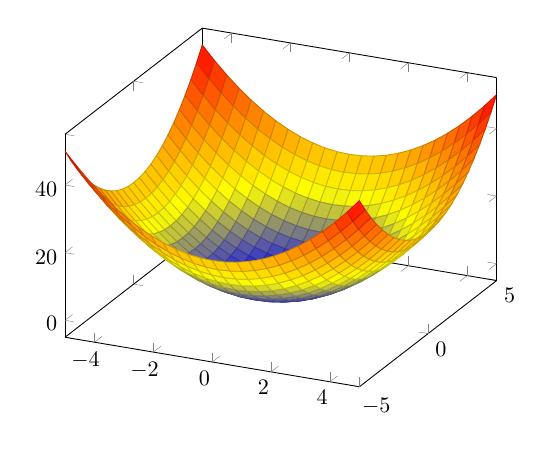
\begin{tikzpicture}[scale = 0.8]
\begin{axis}
\addplot3[
	surf,
]
{x^2 + y^2};
\end{axis}
\end{tikzpicture}
\end{center}

\end{example}


\begin{definition}
Given $f_1, f_2, \ldots f_m \in k[x_1, x_2, \ldots x_n]$, we let 
\begin{align*}
V(f_1, f_2, \ldots f_n) &= V(f_1) \cap V(f_2) \cdots V(f_n) \\
&= \left\{ (a_1, a_2, \ldots a_n) \in \b A^n \mid f_1(a_1, a_2, \ldots a_n) = 0 \text{ and } \cdots \text{ and } f_m(a_1, a_2, \ldots a_n) = 0\right\}
\end{align*}
\end{definition}

\begin{example}
Now consider $f = y - x^2$ and $g = y - x - 2$, then $V(f)$ and $V(g)$ are the following: 

\begin{center}
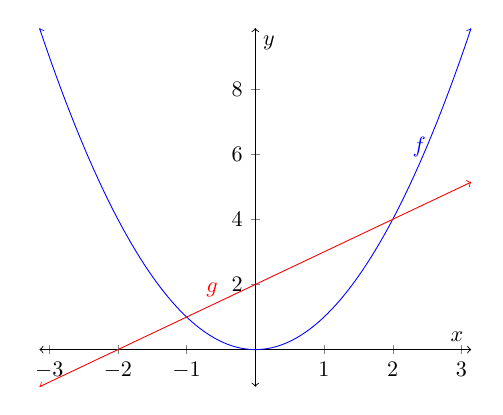
\begin{tikzpicture}[scale = 0.8]
    \begin{axis}[
        axis x line=middle,
        axis y line=middle,
        axis line style=<->,
        xlabel={$x$},
        ylabel={$y$},
        ]
        \addplot[no marks,blue,<->] expression[domain=-pi:pi,samples=100]{x^2} node[pos = 0.8, anchor = south]{$f$}; 
        \addplot[no marks,red,<->] expression[domain=-pi:pi,samples=100]{x + 2} node[pos = 0.4, anchor = south]{$g$}; 
    \end{axis}
\end{tikzpicture}
\end{center}
and the intersection of $V(f)$ and $V(g)$ is preciously $V(f,g) = \left\{ (-1,1), (2,4) \right\}$
\end{example}

\begin{lemma}
Let $S \subset k[x_1, x_2, \ldots x_n]$, 
\begin{enumerate}
 	\item If $f \in S$ and $h \in k[x_1, x_2, \ldots x_n]$, then if $(a_1, a_2, \ldots a_n) \in V(f)$, then $(a_1, a_2, \ldots a_n) \in V(hf)$.
 	\item If $f,g \in S$, then if $(a_1, a_2, \ldots a_n) \in V(f) \cap V(g)$, then $(a_1, a_2, \ldots a_n ) \in V(f + g)$
 \end{enumerate} 
\end{lemma}
\begin{proof}
Since $f(a_1, a_2, \ldots a_n) = 0$, then 
\[(hf)(a_1, a_2, \ldots a_n) = h(a_1, a_2, \ldots a_n)f(a_1, a_2, \ldots a_n) = h(a_1, a_2, \ldots a_n) \cdot 0 = 0.\]
Since $f(a_1, a_2, \ldots a_n) = 0$ and $g(a_1, a_2, \ldots a_n) = 0$, then
\[ (f + g)(a_1, a_2, \ldots a_n) = f(a_1, a_2, \ldots a_n) + g(a_1, a_2, \ldots a_n) = 0 + 0 = 0\]
\end{proof}

\begin{definition}
If $S = k[x_1, x_2, \ldots x_n ]$, we write $I_S$ as the \textbf{ideal generated by } $S$.
\[ I_S = \left\{  h_1 f_1 + h2 f_2 + \cdots + h_m f_m \mid f_1, f_2, \ldots f_m \in S, h_1, h_2, \ldots h_m \in k[x_1, x_2, \ldots x_n ]\right\} \] 
\end{definition}

\begin{corollary}
If $S \subset k[x_1, x_2, \ldots x_n ]$, then $V(S) = V(I_S)$, then vanishing set of $S$ is equal to the vanishing set of $I_S$, the ideal generated by $S$.
\end{corollary}

\begin{definition}
Let $\left( f \right)$ denote the ideal generated by $f$, and let $\left( f_1, f_2, \ldots f_n \right)$ denote the ideal generated by $f_1, f_2, \ldots f_n$, i.e.
\[ \left( f \right) = I_{\left\{ f \right\}}, \left( f_1, f_2, \ldots f_n  \right) = I_{\left\{ f_1, f_2, \ldots f_n \right\}}. \]
\end{definition}

\begin{corollary}
\[ V(f) = V( \left( f \right) )\]
\end{corollary}

\begin{definition}
An \textbf{algebraic subset} of $\b A^n$ is a subset of the form $V(I)$ for some ideal $I \subset k[x_1, x_2, \ldots x_n]$.
\end{definition}

\begin{example}
The \textit{zero ideal} $0 = \left( 0 \right) = \left\{ 0 \right\} \subset k[x_1, x_2, \ldots x_n]$. Thne
\begin{align*}
V(0) &= \left\{ (a_1, a_2, \ldots a_n) \mid (0)(a_1, a_2, \ldots a_n ) = 0 \right\} = \b A^n \\
V(1) &= \left\{ (a_1, a_2, \ldots a_n) \mid (1)(a_1, a_2, \ldots a_n ) = 0 \right\} = \varnothing
\end{align*}
where $(0)$ and $(1)$ are polynomials evaluated at $(a_1, a_2, \ldots a_n)$. 
\end{example}

\begin{example}
For any point $(a_1, a_2, \ldots a_n) \in \b A^n$, the point itself is an algebraic subset. This can be done by construction. Consider the vanishing set of the following polynomial:
\begin{align*}
V(x_1 - a_1, x_2 - a_2, \ldots, x_n - a_n) &= \left\{ (b_1, b_2, \ldots b_n) \in \b A^n \mid b_1 - a_1 = 0, \ldots, b_n - a_n = 0 \right\} \\ 
&= \left\{ (a_1, a_2, \ldots a_n ) \right\}
\end{align*}
\end{example}

\begin{proposition}
Recall

If $I$ and $J$ are ideals of $k[x_1, x_2, \ldots x_n]$, then 
\[ I + J := \left\{ f + g \mid f \in I, g \in J \right\} \text{ and } I \cap J := \left\{ f \mid f \in I \text{ and } f \in J \right\}\]
and both $I + J$ and $I \cap J$ are ideals.
\end{proposition}
\begin{proof}
It's easy to see that $I + J$ and $I \cap J$ are subrings of $k[x_1, x_2, \ldots x_n]$. Now take $f \in I + J$, and let $f_I \in I$ and $f_J \in J$ such that $f_I + f_J = f$ and $h \in k[x_1, x_2, \ldots x_n]$ we have
\begin{align*}
f \cdot h &= (f_I + f_J) \cdot h = f_I \cdot h + f_J \cdot h \in I + J \\
\end{align*}
Now take $g \in I \cap J$, then 
\[ g \cdot h \in I, g \cdot h \in J \implies g \cdot h \in I \cap J \]
\end{proof}
\begin{proposition}[Properties of Ideals]
Let $I, J \in k[x_1, x_2, \ldots x_n]$ be ideals.
\begin{enumerate}
	\item $I \subset J \implies V(J) \subset V(I)$ 
	\item $V(I \cap J) = V(I) \cup V(J)$
	\item $V(I + J) = V(I) \cap V(J)$
\end{enumerate}
\end{proposition}

\begin{proof}
\begin{enumerate}
	\item Say $p = (a_1, a_2, \ldots a_n) \in V(J)$. Then for all $f \in J$ we have $f(p) = 0$. Take any $g \in I \subset J$ we have $g(P) = 0$, therefore $V(J) \subset V(I)$.
	\item ($\subset$) Say $P \not \in V(I) \cup V(J)$, then there exists $f \in I, g \in J$ such that $f(p) \neq 0, g(p) \neq 0$. We then have $fg(p) = f(p) g(p) \neq 0$. Since $fg \in I \cap J$, therefore $p \not\in V(I \cap J)$, taking the contrapositive we have $p \in V(I \cap J) \implies p \in V(I) \cup V(J) \implies V(I \cap J) \subset V(I) \cup V(J)$ \\
	($\supset$) Take $p \in V(I) \cup V(J)$, then without the loss of generality say $p \in V(I)$, then for all $f \in I, f(p) = 0$. Then for all $q \in I \cap J, f(q) = 0 \implies f \in V(I \cap J)$.
	\item ($\subset$)
	($\supset$)
\end{enumerate}
\end{proof}

\begin{example}
Let $I = (x)$ and $J = (y)$, and $I,J \in k[x,y]$. Then we can visualize then on $\b A^2$ in the following figure 
\begin{center}
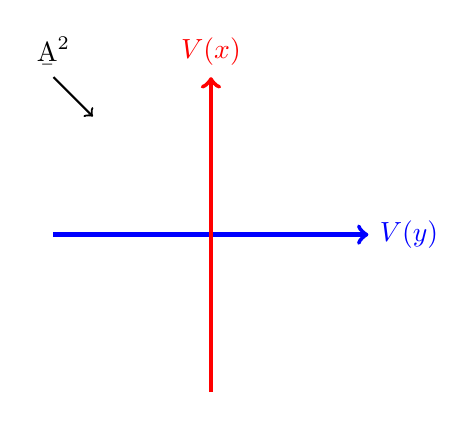
\begin{tikzpicture}
\draw[->,ultra thick, blue] (-2,0)--(2,0) node[right]{$V(y)$};
\draw[->,ultra thick, red] (0,-2)--(0,2) node[above]{$V(x)$};
\draw[<-,thick] (-1.5,1.5) -- (-2,2) node[above]{$\b A^2$};
\end{tikzpicture}
\end{center}
where the red line denotes  $V(x)$ and the blue line denotes $V(y)$.

We have $I \cap J = (x) \cap (y) = (xy)$ (all polynomial divisible by $xy$). Then
\[ V(xy) = \left\{ (x_0, y_0) \mid x_0y_0 = 0 \right\}\]
by inspection we can see that indeed $V(xy) = V(I) \cup V(J)$.

We have $I + J = (x) + (y)$, all polynomials of zero constant terms. Then it's clear to see that
\[ V((x) + (y)) = \left\{ (0,0) \right\}\]
Since there are no constant term in any of the polynomials in $(x) + (y)$. We can also see this is preciously $V(I) \cap V(J)$ too.

\end{example}









